\part{Chiavi duplicate in alberi binari di ricerca}

\begin{tcolorbox}[colback=lightgray!20,%gray background
                  colframe=black,% black frame colour
                  arc=3mm, auto outer arc,]
                  
    \textbf{Esercizio}
    \begin{itemize}
    
    \item Vogliamo confrontare vari modi per gestire chiavi duplicate in ABR:
      \begin{itemize}
        \item implementazione "normale" (senza accorgimenti particolari)
        \item utilizzando un flag booleano
        \item mantenendo una lista di nodi con chiavi uguali
      \end{itemize} 
    \item Per fare questo dovremo:
      \begin{itemize}
        \item Scrivere i programmi Python (no notebook) che:
          \begin{itemize}
            \item implementano quanto richiesto
            \item eseguono un insieme di test che ci permettano di comprendere vantaggi e svantaggi delle diverse implementazioni
          \end{itemize}
          \item Svolgere ed analizzare opportuni esperimenti
          \item Scrivere una relazione (in LATEX) che descriva quanto fatto
          \item Nota: le strutture dati devono sempre essere implementate nel progetto; non si possono utilizzare librerie sviluppate da altri o copiare codice di altri
      \end{itemize}
    \end{itemize}
\end{tcolorbox}

\section{Spiegazione teorica del problema}

\subsection{Introduzione}
\label{sec:Introduzione_1}
In questa sezione vedremo una rapida infarinatura teorica sugli alberi binari di ricerca e sulle operazioni di inserimento e di ricerca. Per i nostri esperimenti
utilizzeremo queste due operazioni poiche' il codice del inserimento lo avremo necessariamente implementato per popolare gli albberi mentre utilizzeremo l'operazione
di ricerca dato che alla base di ogni operazione eseguibile su un ABR c'e' una ricerca (compreso l'inserimento) e quindi i tempi di esecuzione avranno lo stesso andamento per qualsiasi operazione. 


\subsection{Aspetti fondamentali}
\label{sec:AspettiFondamentali_1}

Un albero binario di ricerca (esempio in figura \ref{fig:ABR}) e' un tipologia particolare di albero binario con le seguenti caratteristiche:
\begin{enumerate}
    \item Il sottoalbero sinistro di un nodo $x$ contiene soltanto i nodi con chiavi minori della chiave del nodo $x$.
    \item Il sottoalbero destro di un nodo $x$ contiene soltanto i nodi con chiavi maggiori della chiave del nodo $x$.
    \item Il sottoalbero destro e il sottoalbero sinistro devono essere entrambi due ABR.
\end{enumerate}
Descriviamo ora le caratteristiche delle due operazioni che prenderemo in considerazione:

\begin{itemize}
  \item Per l'inserimento, iniziando dalla radice dell'albero, si sceglie ricorsivamente su quale ramo spostarsi basandoci sul confronto tra la chiave della foglia in cui
  siamo e il valore che vogliamo inserire. Arrivati in fondo all'albero creeremo un nuovo nodo (se destro o sinistro rispetto all'ultima foglia dipende 
  dall'implementazione.
  Vediamo ora la differenza tra le varie implementazioni che andremo adanalizzare, tenendo a mente che esse si differenziano solo per come gestiscono le chiavi    
  duplicate mentre hanno lo stesso comportamento negli altri casi (inserimento destro se la chiave del nuovo node e maggiore e sinistro se la chiave e minore).
    \begin{itemize}
      \item Classica
      \item Flag booleana
      \item Lista concatenta di nodi con chiavi uguali
    \end{itemize}
  \item Nel operazione di ricerca per ogni foglia prima confrontiamo il valore che stiamo cercando con quella della suddetta foglia. Se il valore è uguale allora ritorneremo
  un boolean di conferma. Se raggiunta l'ultima foglia dell'albero non trovassimo il valore allora ritorneremo un boolean di fallimento. Altrimenti se non ci
  troviamo in nessuna delle due situazioni appena descritte scendiamo l'albero con lo stesso metodo dell'inserimento. Ovviamente per fare la ricerca partiremo
  dalla radice dell'albero.
\end{itemize}

\begin{figure}[H]
  \centering
  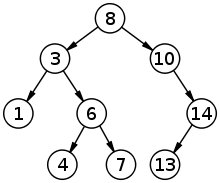
\includegraphics[width=0.35\textwidth]{Resources/ABR_RN_Resources/ABR.png}
  \caption{Albero binario di ricerca}
  \label{fig:ABR}
\end{figure}

\subsection{Assunti ed ipotesi}
\label{sec:AssuntiEdIpotesi_1}
In un ABR le operazioni di base richiedono un tempo proporzionale all'altezza dell'albero. L'altezza attesa di un ABR costruito in modo casuale è $O(h)$ quindi
le operazioni elementari svolte su questo tipo di albero richiedono in media $\Theta(h)$. Nel caso peggiore, il caso in cui l'albero sia completamente sbilanciato 
da un lato, dando cosi origine ad una lista, l'altezza è $\Theta(n)$ e quindi ci aspettiamo che le operazioni elementari richiedano $\Theta(n)$ per essere svolte.
Per vedere la complessità degli algoritmi più importanti di ABR basati sul caso peggiore e sul caso medio si richiama alla figura \ref{fig:ComplessitàABR} facendo
particolare attenzione ai metodi in rosso che sono quelli su cui andremo a svolgere gli esperimenti.
Poiche andremo a sperimentare su varie metodologie di inserimento e utile ipotizzare come questi avranno impatto sulle prestazioni del albero. In particolare
ci aspettiamo di vedere, in caso di un elevato numero di chiavi ripetute, una migliore prestazione nella ricerca, dovuta alla ridotta altezza del albero per quanto riguarda il metodo
di inserimento basato sulla lista concatenata e allo stesso modo un altezza inferiore anche per il metodo con flag booleana che dovrebbe rendere piu bilanciat l'albero 
e quindi ridurne l'altezza. 
Al contrario il maggior numero di operazioni necessare dovrebbe rendere il metodo con lista, il piu lento nel inserimento di nuovi dati.

\begin{figure}[H]
    \centering
    \begin{tabular}{|c|c|c|}
        \hline
         & Complessità al caso peggiore & Complessità al caso medio\\
        \hline
        Spazio & $\Theta$($n$) & $\Theta$($n$)\\
        \hline
        \textcolor{red}{Inserimento} & $O(n)$ & $O(h)$\\
        \hline
        \textcolor{red}{Ricerca} & $O(n)$ & $O(h)$\\
        \hline
        Cancellazione & $O(n)$ & $O(h)$\\
        \hline
    \end{tabular}
    \caption{Complessità degli algoritmi di ABR}
    \label{fig:ComplessitàABR}
\end{figure}
Il nostro obiettivo in questo test è verificare sperimentalmente la veridicità delle varie complessità descritte nella figura \ref{fig:ComplessitàABR} e capire
sotto quali condizioni un albero è più conveniente di un altro confrontandoli, a parità di numero di chiavi, in base al tempo reale che impiegano ad eseguire le operazioni.

\newpage
\section{Documentazione del codice}

\subsection{Schema del contenuto e interazione tra i moduli}
\label{sec:SchemaContenutoInterazioneModuli_1}
Per svolgere i nostri esperimenti ho, prima di tutto, scritto il codice delle strutture dati a cui faremo riferimento. In questo caso le classi hanno nome \textbf{ABR} per gli alberi binari di ricerca e \textbf{RN} per gli alberi rosso neri. Le classi \textbf{Node} e \textbf{NodeRN} sono le classi che descrivono i nodi. La classe \textbf{Node} è pensata per essere 'usata' dalla classe \textbf{ABR} mentre la classe \textbf{NodeRN} per \textbf{RN}. Notiamo che \textbf{RN} è una sottoclasse di \textbf{ABR} per il semplice motivo che gli alberi rosso neri sono degli alberi binari di ricerca con specifiche regole in più descritte nel capitolo \ref{sec:AspettiFondamentali_1}. Stessa cosa vale per le classi \textbf{Node} e \textbf{NodeRN} (\textbf{NodeRN} è una sottoclasse di \textbf{Node}). Entrambe le tipologie di nodi si aggregano con i rispettivi alberi (Basta solo l'istanza del nodo della radice). Importante notare come la classe \textbf{Node} (e quindi conseguentemente la classe \textbf{NodeRN}) abbia un vincolo di aggregazione ricorsivo di moltiplicità 3. Questo è dovuto al fatto che un oggetto della classe \textbf{Node} deve avere al suo interno le istanze del nodo padre e dei nodi figli. 

\begin{figure}[H]
    \centering
    \includegraphics[width=0.8\textwidth]{Resources/ABR_RN_Resources/ABR_RN_UML_1.png}
    \caption{Diagramma delle classi ABR e RN}
    \label{fig:ABR_RN_UML_1}
\end{figure}

In più ho creato una classe semplicemente al fine di svolgere questo esperimento. \textbf{PlotGenerator} è una classe utile per la generazione di infografiche utili per vedere la funzione che si evolve nel tempo dei due metodi che andrò ad analizzare.

\begin{figure}[H]
    \centering
    \includegraphics[width=0.7\textwidth]{Resources/ABR_RN_Resources/ABR_RN_UML_2.png}
    \caption{Diagramma della classe PlotGenerator}
    \label{fig:ABR_RN_UML_2}
\end{figure}

\subsection{Analisi delle scelte implementative}
\label{sec:AnalisiScelteImplementative_1}
Con la descrizione delle varie classi e delle interazioni tra loro vanno comprese anche alcune delle scelte implementative utili al funzionamento delle strutture dati in questione. Partendo dalla classe \textbf{RN} si può notare l'attributo \textit{sent}. In questo attributo instanzieremo un oggetto di tipo \textbf{NodeRN} con le seguenti qualità:

\begin{itemize}
    \item nessun padre
    \item colore nero
    \item chiave -1
\end{itemize}

Questa sentinella sarà usata come 'padre' della radice e come 'figlio' di tutti quei nodi che non hanno qualcuno dei 'figli'. Ho inserito anche un attributo \textit{dim} nelle classi degli alberi che servirà per il calcolo delle infografiche. Per il resto non ci sono grandi differenze implementative rispetto a quello che un qualsiasi libro di Algoritmi e Strutture Dati introduce.

\subsection{Descrizione dei metodi implementati}
\label{sec:DescrizioneMetodiImplementati_1}
In questa parte descriverò le funzionalità di ogni metodo delle classi di cui finora abbiamo parlato. 

\begin{itemize}

    \item \textbf{Node}
    \begin{itemize}
    
        \item \textbf{getP()} : restituisce il nodo padre \textit{p}.
        
        \item \textbf{getKey()} : restituisce l'attributo \textit{key}.
        
        \item \textbf{getName()} : restituisce la stringa \textit{name}.
        
        \item \textbf{setKey(key)} : modifica l'attributo \textit{key} della classe con il valore del parametro.
        
        \item \textbf{getChildren()} : restituisce un array di nodi (più precisamente \textit{left} e \textit{right} in quest'ordine).
        
        \item \textbf{toString()} : stampa a schermo gli attributi del nodo.
        
    \end{itemize}
    
    \item \textbf{NodeRN}
    \begin{itemize}
        \item come sottoclasse di \textbf{Node} può usare tutti i metodi della superclasse e fare override di alcuni di essi.
        
        \item \textbf{getColor()} : restituisce la stringa \textit{color}.
        
        \item \textbf{setColor(color)} : modifica la stringa \textit{color} della classe con il valore del parametro.
        
        \item \textbf{toString()} : stampa a schermo gli attributi del nodo più l'attributo color.
        
    \end{itemize}
    
    \item \textbf{ABR}
    \begin{itemize}
        \item \textbf{setRoot(key)} : instanzia un oggetto \textbf{Node} su \textit{root}.
        
        \item \textbf{insert(key)} : chiama il metodo \textbf{setRoot(key)} se \textit{root} è NULL altrimenti chiama il metodo \textbf{insertNode(currentNode, key)}. Incrementa \textit{dim}.
        
        \item \textbf{insertNode(currentNode, key)} : attraversa l'albero ricorsivamente fino a che non trova una foglia libera. A questo punto crea un istanza di \textbf{Node} con chiave \textit{key}.
        
        \item \textbf{find(key)} : ritorna il valore del metodo \textbf{findNode(self.root, key)}.
        
        \item \textbf{findNode(currentNode, key)} : attraversa l'albero ricorsivamente e se trova un nodo con valore uguale a \textit{key} allora ritorna TRUE altrimenti ritorna FALSE.
        
        \item \textbf{take(key)} : ritorna il valore del metodo \textbf{takeNode(self.root, key)}.
        
        \item \textbf{takeNode(currentNode, key)} : attraversa l'albero ricorsivamente e se trova un nodo con valore uguale a \textit{key} allora ritorna \textit{currentNode} altrimenti ritorna FALSE.
        
        \item \textbf{inorder()} : stampa a schermo tramite un attraversamento simmetrico dell'albero tutti gli attributi dei nodi dell'albero.
        
        \item \textbf{minimum()} : restituisce NULL se l'attributo \textit{root} è NULL altrimenti chiama \textbf{searchMin(self.root)}.
        
        \item \textbf{searchMin(currentNode)} : scende ricorsivamente l'albero usando come attributo \textit{currentNode.left}. Se con la verifica \textit{currentNode.left} è NULL allora restituisce \textit{currentNode}.
        
        \item \textbf{maximum()} : restituisce NULL se l'attributo \textit{root} è NULL altrimenti chiama \textbf{searchMax(self.root)}.
        
        \item \textbf{searchMax(currentNode)} : scende ricorsivamente l'albero usando come attributo \textit{currentNode.right}. Se con la verifica \textit{currentNode.right} è NULL allora restituisce \textit{currentNode}.
        
        \item \textbf{successor(currentNode)} : restituisce l'oggetto di tipo \textbf{Node} con chiave \textit{key} con il valore immediatamente successivo al valore della chiave di \textit{currentNode} all'interno dell'albero.
        
        \item \textbf{predecessor(currentNode)} : restituisce l'oggetto di tipo \textbf{Node} con chiave \textit{key} con il valore immediatamente precedente al valore della chiave di \textit{currentNode} all'interno dell'albero.
        
        \item \textbf{transplant(oldNode, subNode)} : sostituisce il sottoalbero con radice \textit{oldNode} con il sottoalbero di radice \textit{subNode}.
        
        \item \textbf{delete(currentNode)} : chiama il metodo \textbf{transplant(oldNode, subNode)} per la sostituzione del sottoalbero mantenendo la validità delle proprietà dell'ABR.
        
    \end{itemize}
    
    \item \textbf{RN}
    \begin{itemize}
    
        \item come sottoclasse di \textbf{ABR} può usare tutti i metodi della superclasse e fare override di alcuni di essi.
        
        \item \textbf{setRoot(key)} : instanzia un oggetto \textbf{Node} su \textit{root} che avrà come padre e figli l'attributo \textit{sent}.
        
        \item \textbf{leftRotate(currentNode)} : operazione locale che effettua una rotazione tra \textit{currentNode} e \textit{currentNode.right}.
        
        \item \textbf{rightRotate(currentNode)} : operazione locale che effettua una rotazione tra \textit{currentNode} e \textit{currentNode.left}.
        
        \item \textbf{rbInsertFixup(currentNode)} : modifica della struttura dell'albero che usa i due metodi \textbf{leftRotate(currentNode)} e \textbf{rightRotate(currentNode)} oltre a modificare gli attributi \textit{color} dei vari nodi secondo le regole dello RN.
        
        \item \textbf{insertNode(currentNode, key)} : simile al metodo di \textbf{ABR} con la chiamata del metodo \textbf{rbInsertFixup(currentNode)} alla fine.
        
        \item \textbf{delete(currentNode)} : metodo non implementato. Restituisce NULL.
        
    \end{itemize}
    
    \item \textbf{PlotGenerator}
    \begin{itemize}
    
        \item \textbf{createTree(treeType)} : restituisce un'istanza di una delle tipologie di albero. Se \textit{treeType} è FALSE restituisce un'istanza di un oggetto \textbf{ABR} viceversa se TRUE restituisce un'istanza di un oggetto \textbf{RN}.
        
        \item \textbf{insertTimeTest(n, tree, caseSelect, timeCalculation, randomRange=5000)} : restituisce una lista di float contenente i tempi che ci vogliono per l'esecuzioni in serie del metodo \textbf{insert(key)}. Se \textit{caseSelect} è FALSE prenderemo il caso della catena lineare viceversa il caso randomico se TRUE. Nel caso randomico i numeri che verrano generati all'interno dell'albero andranno da 0 a \textit{randomRange}. Se \textit{timeCalculation} è FALSE il calcolo del tempo avviene tramite la differenza tra il tempo di fine e il tempo di inizio più il tempo precedentemente registrato nell'array viceversa il calcolo del tempo avviene tramite la differenza tra il tempo di fine e il tempo di inizio diviso la dimensione dell'albero \textit{dim} più il tempo precedentemente registrato nell'array se TRUE.
        
        \item \textbf{searchTimeTest(n, tree, caseSelect, timeCalculation, randomRange=5000)} : restituisce una lista di float contenente i tempi che ci vogliono per l'esecuzioni in serie del metodo \textbf{find(key)}. Il funzionamento di \textit{caseSelect}, \textit{timeCalculation} e \textit{randomRange} è uguale ad \textbf{insertTimeTest(n, tree, caseSelect, timeCalculation, randomRange=5000)}.
        
        \item \textbf{generatePlot(timeArray, graphType, nameGraph)} : genera un infografica che rappresenta la funzione nel tempo data da \textit{timeArray}. \textit{nameGraph} è il nome che verrà assegnato al grafico. \textit{graphType} offre due tipi di rappresentazione per il grafico: se FALSE offre una rappresentazione continua viceversa discreta se TRUE.
        
        \item \textbf{confrontatePlot(superTimeArray, nameGraph, listLabel)} :  genera un infografica data da più funzioni. Il numero di funzioni è uguale alla dimensione di \textit{superTimeArray}. Simile a \textbf{generatePlot(timeArray, graphType, nameGraph)} ma con un solo tipo di rappresentazione, quella continua. \textit{listLabel} è una lista contenente i nomi di ogni label che vanno assegnanati alle funzioni.
        
        \item \textbf{generateSuperPlot(superTimeArray)} : genera delle infografiche con tutti i possibili confronti utili alla nostra sperimentazione. \textit{superTimeArray} è la lista che contiene tutti i \textit{timeArray} elementari (cioè tutte le possibili combinazioni esistenti).
        
    \end{itemize}
    
\end{itemize}

\newpage
\section{Descrizione degli esperimenti condotti e analisi dei risultati sperimentali}

\subsection{Dati utilizzati}
\label{sec:DatiUtilizzati_1}
Per gli esperimenti che andremo ad eseguire utilizzeremo diversi tipi di dataset per poter coprire il maggior numero possibile di casi che 
si potrebbero incontrare nel effettivo utilizzo di questi algoritmi. Un dataset di test e costituito da un insieme di "sotto-dataset" che rendono i test completi.
Il dataset e' quindi coposto da 3 tipi di array:
\begin{itemize}
  \item Random Dataset (RD) ovvero dataset di interi generati casualmente con numeri tra 0 e la dimensione del array
  \item High Repetitions Dataset (HRD) ovvero dataset di interi generati casualmente con numeri tra 0 e la meta della dimensione del array, cosi da aumentare il numero di ripetizioni 
  \item Worst Case Dataset (WCD) ovvero un HRD ordinato in modo crescente, cosi da ottenere un albero completamente sbilanciato
\end{itemize}

Ognuno di questi array viene generato in diverse dimensioni ( 100, 200, 300,...,1000 elementi ) in modo da poter vedere la complessita delle operazioni 
al crescere del dataset.
Infine ognuno di questi test viene eseguito 500 volte, per poter minimizzare l'errore dovuto a fattori esterni al programma calcolando
la media del tempo impiegato per ogni test.

\subsection{Misurazioni}
\label{sec:Misurazioni_1}
La funzione di benchmark riceve in input il dataset su cui deve eseguire il test e il metodo di inserimento che dovra
testare. Per ogni array nel dataset quindi costruisce un albero con il metodo di inserimento specificato tralasciando l'ultimo elemento.
Procedera poi a cronometrare il tempo impiegato per l'inserimento del ultimo elemento simulando percio il tempo impiegato ad 
inserire un dato in un albero gia costruito.
In seguito cronometra la ricerca di un intero generato casualmente tra 0 e la dimensione del array fratto 10, cosi che la possibilita di una ricerca con successo
sia maggiore ma lasciando comuqnue la possibilita di una ricerca falllita.
Questi test vengono eseguiti come detto in precedenza 500 volte per ogni dimensione e viene calcolata una media per ogni dimensione ottenendo come output due array.
Un array contenente la media dei tempi di inserimento per ogni dimensione e uno contenente la media dei tempi di ricerca per ogni dimensione. 

\subsection{Risultati sperimentali e commenti analitici}
\label{sec:RisultatiSperimentaliCommentiAnalitici_1}

\subsubsection{Inserimento}
Iniziamo subito notando come i risultati del test che vediamo in figura \ref{fig:RDHDins} confermino quanto ipotizzato dalla nostra analisi teorica \ref{sec:AssuntiEdIpotesi_1}
ottenendo ... come andamento delle operazioni di inserimento su dataset RD e HRD che rappresentano il caso medio.
Andando piu in dettaglio con l'analisi possiamo notare come i casi medi indifferentemente dal tipo di dataset abbaino un andamento molto simile a parita di
algoritmo utilizzato per l'inserimento coronando l'algoritmo classico come il piu rapido seguito poi dalla lista concatenata e infine dalla flag booleana. 
A differenza di quanto potesse essere ipotizzabile, data la maggiore complessita delle operazioni per la creazione della lista concatenata, l'algoritmo con lista
risulta piu prestante di quello booleano probabilmente aiutato dal fatto che incorporando i nodi simili in uno solo riduce l'altezza del albero e quindi il numero di 
cicli necessari per l'inserimento, a differenza della flag booleana che si limita a cercare di bilanciare meglio l'albero, mantenendo pero il numero di nodi invariato.


\begin{figure}[H]
  \centering
  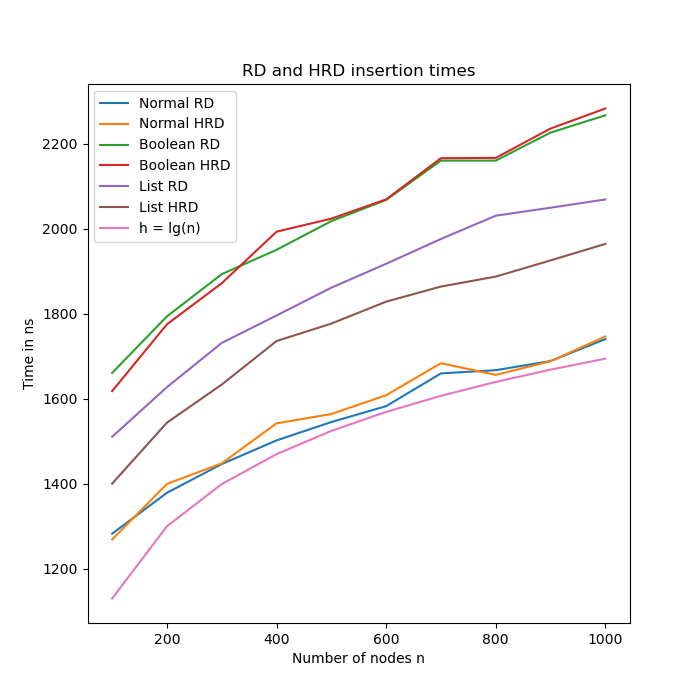
\includegraphics[width=0.5\textwidth]{Resources/ABR_Resources/RDeHRDinsertion.png}
  \caption{Inserimento su RD e HRD}
  \label{fig:RDHDins}
\end{figure}


Anche per quanto riguarda i risultati mostrati in figura \ref{fig:WCDins} possiamo notare come gli esperimenti abbiano comfermato la nostra analisi teorica mostrando
un andamento ... per tutti gli algoritmi nel caso peggiore. Non ci sorprende vedere come l'algoritmo basato sulla lista concatenata risulti il piu rapido in quanto
riducendo il numero di nodi riduce anche l'altezza del albero (che nel caso peggiore risulta essere una lista) permettendo cosi di ottenere i risultati migliori.
Risulta interessante pero notare come l'algoritmo classico risulti piu prestante di quello con flag booleana.
\begin{figure}[H]
  \centering
  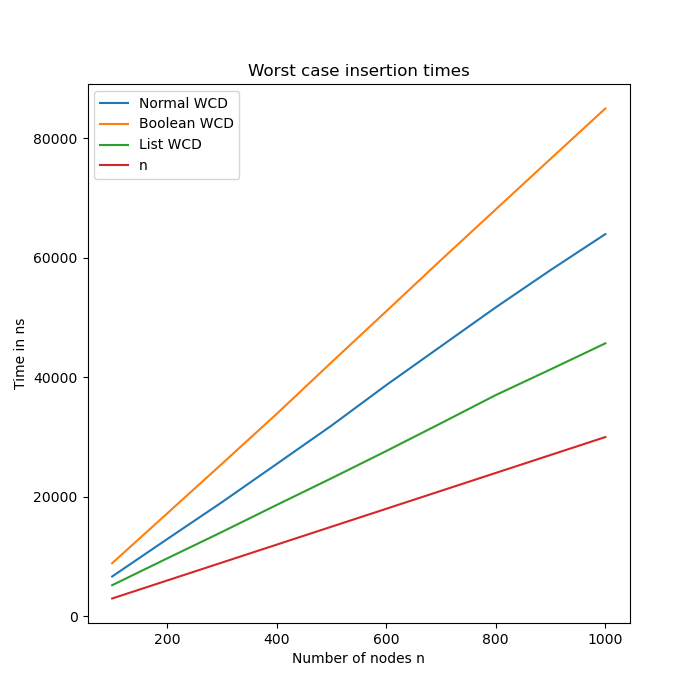
\includegraphics[width=\textwidth]{Resources/ABR_Resources/WDinsertion.png}
  \caption{Ricerca}
  \label{fig:WDins}
\end{figure}

\subsubsection{Ricerca}

Per quanto riguarda le prestazioni della ricerca mostrate in figura \ref{fig:RDHRDsearch} possiamo notare come i risultati sperimentali abbiano confermato le nostre
ipotesi con un andamento ... per i dataset RD e HRD.
Salta subito al occhio come tutti gli algoritmi abbiano prestazioni migliori nel caso di dataset ad alte ripetizioni dato dal fatto che sono stati ottimizzati 
appositamente per questa evenienza e non ci sorprende vedere come sia su dataset RD che HRD l'algoritmo con lista concatenata risulti il piu prestante.
Aggiungiamo inoltre che su dataset RD le prestazioni sono quasi identiche per tutti gli algoritmi con un leggero miglioramento per quanto riguarda l'algoritmo
a lista condatenata mentre per i dataset HRD l'algoritmo a lista concatenata risulta decisamente piu prestante rispetto agli altri due che danno risultati molto simili.

\begin{figure}[H]
  \centering
  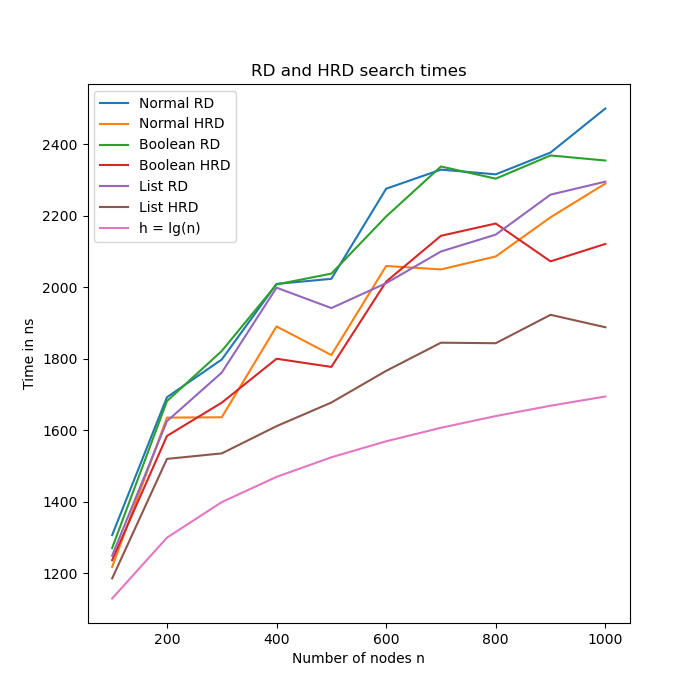
\includegraphics[width=0.5\textwidth]{Resources/ABR_Resources/RDeHRDsearch.png}
  \caption{Ricerca su RD e HRD}
  \label{fig:RDHRDsearch}
\end{figure}

Come per i casi precedenti anche su dataset WCD i risultati in figura \ref{fig:wdcsearch} sono concordanti con la nostra previsione di una complessita ... .
Nuovamente l'algoritmo con lista concatenata risulta nettamente piu prestante degli altri anche se vediamo un leggero miglioramento di prestazioni da parte 
del algoritmo con flag booleana rispetto a quello con implementazione classica.
\begin{figure}[H]
  \centering
  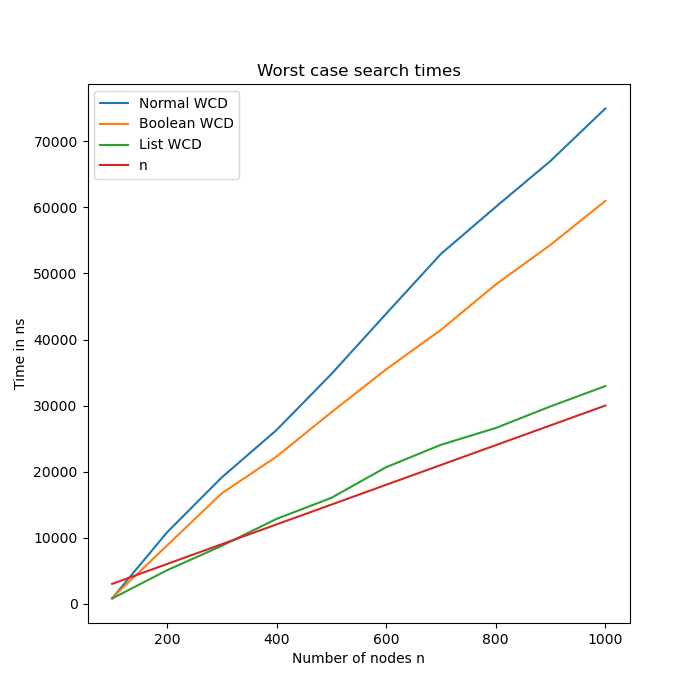
\includegraphics[width=0.5\textwidth]{Resources/ABR_Resources/WDsearch.png}
  \caption{Ricerca su WCD}
  \label{fig:wdcsearch}
\end{figure}

\subsection{Tesi e sintesi finale}
\label{TesiSintesiFinale_1}
Come già descritto nella sezione \ref{sec:RisultatiSperimentaliCommentiAnalitici_1} possiamo dare le seguenti conclusioni:
\begin{itemize}
    \item I metodi inserimento e ricerca nel caso della catena lineare con albero ABR hanno complessità $\Theta(n)$. In tutti gli altri casi descritti la complessità è $O(h)$.
    \item I metodi inserimento e ricerca nel caso della catena lineare con albero ABR ci mettono un tempo esponenziale all'aumentare del numero di nodi inseriti basato sulla formula \ref{eqn:timeArray1} della sezione \ref{sec:Misurazioni_1}. Tutti gli altri metodi ci mettono tempo lineare sempre basato sulla formula \ref{eqn:timeArray1}.
    \item Nel caso dell'inserimento randomico si può notare che ABR è migliore di RN (Questo è probabilmente dovuto al riequilibrio dell'albero RN). Questa tendenza sembra invertirsi nel caso della ricerca randomica (Infatti avendo riequilibrato in albero in media ci vorrà meno tempo a cercare un nodo all'interno di un RN rispetto ad un ABR). Questo fa notare che il riequilibrio dell'albero RN può essere utile per lo svolgimento di alcune operazioni che potrebbero metterci molto più tempo senza riequilibrio.
    \item Il tempo delle operazioni randomiche non sembra variare significativamente a seconda del range di numeri che possono essere usati come chiave nei nodi degli alberi. L'affermazione precedente è dovuta al fatto che dopo aver effettuato un numero elevato di test non si è rilevato un aumento o un decremento eccessivo nei tempi dati dalle varie mediane calcolate per ogni tipologia di operazione valutata.
\end{itemize}



